\subsection{Parameteroptimierung}

Da sich nun keine implementationstechnischen Fehler mehr im Programm befinden, können wir dazu übergehen die unterschiedlichen Parameter so anzupassen, dass die Karte eines durch Pappkartons errichteten Bereiches im Labor optimal aufgenommen wird.

\subsubsection{Optimierung des COUNT-Parameters (Jan)}

Der COUNT-Parameter legt fest bei welchen Schleifendurchläufen zusätzlich zur Hindernisvermeidung auch ein Karten-Update durchgeführt wird. Dies ist zum einen notwendig, damit der Roboter mit den Scans hinterherkommt und zum anderen sinnvoll, da der Roboter dann bereits eine bedeutendere Bewegung durchgeführt hat, sodass in der Differenz der Scans die Bewegungsänderung signifikanter als das Rauschen ist. Wir haben zusätzlich einen kurzen Sleep von 100ms in die Hauptschleife eingefügt, damit der Roboter mit den Scans nicht in Verzug gerät, aber trotzdem zeitnah auf auftauchende Hindernisse reagieren kann.
Wir haben den COUNT-Parameter im Bereich von 2 bis 8 getestet. Die besten Ergebnisse bekamen wir bei einem COUNT von 4, was bedeutet, dass in jedem 4. Schritt ein Karten-Update durchgeführt wird.

%TODO bilder?

\section{Aktualisieren des Referenzscans}

\subsubsection{Auflösung der Histogramme (Jan)}

Ein weiterer wichtiger Parameter ist die Auflösung der Histogramme.
Für das Winkelhistogramm ist natürlich wichtig, dass eine Rotation möglichst genau abgebildet werden kann. Falls ein Maximum sich aber auf mehrere Bins aufteilt, kann es sein, dass das Maximum nicht gefunden wird. Hier ist es deshalb wichtig einen guten Mittelweg zu finden. Initial haben wir für die Winkelhistogramme eine Binanzahl von 300 gewählt, was einer Auflösung von 1,2 Grad pro Bin entspricht. Im weiteren Verlauf haben wir die Binanzahl auf 400 erhöht, was eine leichte Verbesserung mit sich brachte. Eine Erhöhung der Binanzahl auf 500 hatte wiederum eine Verschlechterung zur Folge. Mit einer Anzahl von 550 Bins für das Winkelhistogramm haben wir letztendlich die besten Ergebnisse erzielen können. Dies entspricht einer Auflösung von etwa 0,65 Grad pro Bin.

\begin{figure}
	\centering
	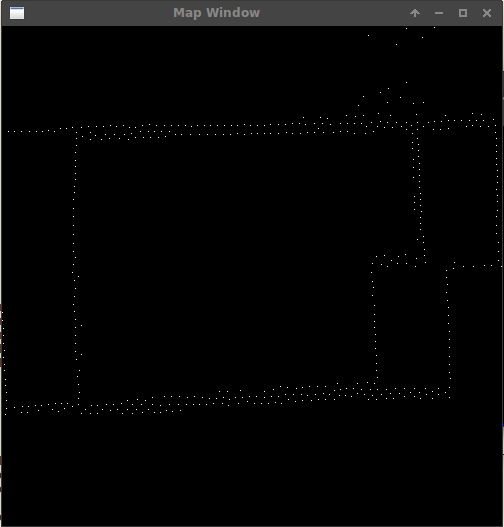
\includegraphics[width=10cm]{netzwerk}
	\caption{Verrutschen der Karte, vermutlich verursacht durch eine Netzwerkverzögerung}
	\label{fig:netzwerk}
\end{figure}

Die Anzahl der Bins für die X- und Y-Histogramme muss zusätzlich auch immer noch auf die Distanzen in der Umgebung angepasst werden. Die optimalen Ergebnisse auf dem Roboter im Testbereich im Labor erzielten wir mit 500 Bins und einer maximalen Distanz von 6 Metern. Dies entspricht einer Auflösung von 1,2 cm pro Bin.

\subsubsection{Verrutschen der Karte (Jan)}

Ab und zu kam es zu einem verrutschen der Karte. Wir nehmen an, dass hier durch eine Verzögerung des Netzwerks ein Scan zum falschen Zeitpunkt eingezeichnet wurde. Dieses Problem trat allerdings sehr selten auf und konnte auch an keinem weiteren Faktor festgemacht werden. Wie in Abbildung~\ref{fig:netzwerk} zu sehen ist, ist dadurch natürlich die Karte ungültig und es muss ein neuer Versuch gestartet werden.
